%% International Journal of Computational Intelligence Systems ---
%%%%%%%%%%%%%%%%%%%%%%%%%%%%%%%%%%%%%%%%%%%%%%%%%%%%%%%%%%%%%%%%%%%%%%%%%%%
\documentclass[11pt,twoside]{article}
\usepackage{ijcis}
%--------------------- ADDITIONAL PACKAGES HERE ---------------------------
\usepackage{lscape}
\usepackage{pdflscape}
\usepackage{setspace}
\usepackage{afterpage}
\usepackage{alltt}
%--------------------------------------------------------------------------
%
\def\labart{jFuzzyLogic}    % put a label from your choice here
%\Vol{1}                    % number of the Volume
%\Issue{1}                  % number of the issue
%\Month{January}            % month
%\Year{2008}                % year
%\received{...}
%\revised{...}
%
%---------------------------------------------------------------------------
\thispagestyle{empty}
%%------------------------- YOUR HEADINGS HERE -----------------------------
% Author's initials of first names+last names
\shortauthors{Pablo Cingolani, Jes\'us Alcal\'a-Fdez}
% Short title
\shorttitle{jFuzzyLogic}
%---------------------------------------------------------------------------
%
%---------------------- YOUR TITLE ----------------------------------------
\title{Rapid development of fuzzy logic control using jFuzzyLogic}
%-------------------------- AUTHOR'S NAMES ----------------------------------
\author{%
Pablo Cingolani\,\up{1},
%\author{
Jes\'us Alcal\'a-Fdez\,\up{2}
}
%----------------------------- ADDRESSES ----------------------------------
\addresses\address{%
\\ \vspace*{0.05truein}
\up{2}
Department of Computer Science and Artificial Intelligence, University of Granada,\\
Research Center on Information and Communications Technology,\\
C/ Periodista Daniel Saucedo Aranda s/n,\\ 
Granada, 18071, Spain
\\ \vspace*{0.04truein}
E-mail: jalcala@decsai.ugr.es
}
%---------------------------------------------------------------------------
\pagestyle{myheadings}
\begin{document}
\label{\labart-FirstPage}

\maketitle
%-------------------------- ABSTRACT ---------------------------------------
\abstracts{%
This work introduces jFuzzyLogic, a software framework that allows for rapid development of fuzzy systems.
JFuzzyLogic's goal to facilitate and accelerate development of fuzzy systems is achieved by
i) using standard programming language that reduces learning curves; 
ii) providing a fully functional and complete implementation of fuzzy inference system; 
iii) creating an API that developers can use or extend;
iv) implementing an Eclipse plugin to easily write and test FCL code;
v) making the software platform independent; 
and vi) distributing the software as open source.
The use of jFuzzyLogic is illustrated through the analysis of one case study.
}
\par\bigskip\par
%-------------------------- KEYWORDS ---------------------------------------
\keywords{List of four to six keywords which characterize the article.}

\vspace*{10pt}\textlineskip
%-------------------------- BEGIN BODY OF TEXT -----------------------------
\begin{multicols}{2}

%--------------------------------------------------------------------------
\section{Introduction}
%--------------------------------------------------------------------------

Fuzzy rule based systems (FRBSs) are one of the most important areas for the application of the Fuzzy Set Theory\cite{Zadeh65}. 
%Usually it is considered a model structure in the form of 
Classical rule based systems deal with IF-THEN rules.
FRBSs constitute an extension to classical systems, having antecedents and consequents composed of fuzzy logic statements.

A Fuzzy Logic Controller (FLC)~\cite{Lee90,DHR93,YF94,Bon94} is a FRBS composed of: 
	i-) a Knowledge Base that comprises the information used by the expert operator in the form of linguistic control rules; 
	ii-) a Fuzzification Interface, that transforms the crisp values of the input variables into fuzzy sets;
	iii-) an Inference System, that uses the fuzzy values from the Fuzzification Interface and the information from the Knowledge Base to perform the reasoning process and 
	iv-) the Defuzzification Interface, which takes the fuzzy action from the Inference System and translates it into crisp values for the control variables.

FLCs are suitable for engineering applications in which classical control strategies do not achieve good results or when it is too difficult to obtain a mathematical model.
FLCs usually have two characteristics: the need for human operator experience, and a strong non linearity.
Many real-world applications use FLCs~\cite{PDH97} such as mobile robot navigation \cite{MAA10,JCh2011}, air conditioning controllers \cite{Alc12,Cho11}, domotic control\cite{Cha12,AL05}, and industrial applications\cite{ZG2012,Demir12}.
0
FLCs are powerful for solving a wide range of problems, but their implementation requires a certain programming expertise.
In the last few years, many fuzzy logic software tools have been developed to reduce this task. 
Some are commercially distributed, for example MATLAB Fuzzy logic toolbox(www.mathworks.com), while a few are available as open source software (see section \ref{sec:stu}).

In this work, we introduce an open source Java library named jFuzzyLogic. 
This fuzzy systems library allows FLCs design and implementation, following the standard for Fuzzy Control Language (FCL) published by the International Electrotechnical Commission (IEC 61131-7)\cite{IEC}. 

The main goal of jFuzzyLogic is to bring the benefits of open source software and standardization to the fuzzy systems community. Our library offers several advantages:

\begin{itemize}

	\item Standardization, which reduces programming work and learning curve. This library contains the basic programming elements for the Standard IEC 61131-7, alleviating developers from boiler plate programming tasks.

	\item Extensibility, the object model and API allows to create a wide range of applications. This is of special interest for the research community.

	\item Platform independence, allows to develop and run on any hardware and operating system configuration that supports Java.

\end{itemize}

This work is arranged as follows.
The next section presents a comparison on non-commercial fuzzy software and the main benefits that the jFuzzyLogic offers with respect to other libraries. 
Section~\ref{sec:IEC} introduces the concepts of IEC standard (IEC-61131) control programming languages.
Section~\ref{sec:jFu} describes jFuzzyLogic's main features. 
Section~\ref{sec:cas}, illustrates how jFuzzyLogic can be used in a control application.
Conclusions are presented in Section~\ref{sec:con}.

%--------------------------------------------------------------------------
\section{Comparison of fuzzy logic software\label{sec:stu}}
%--------------------------------------------------------------------------

In this section we present a comparison on non-commercial fuzzy software (Table~\ref{t:comp}).
We center our interest on free software distributions because of its important role in the scientific research community~\cite{Sonnenburg07}.
Moreover, we do not want to establish a comparison among all software tools or to emphasize the advantages of one over another.
Our objective is to detect the major differences in the software and then to categorize jFuzzyLogic as an alternative to these suites when other research requirements are needed.

We analyze twenty five packages (including jFuzzyLogic), mostly from SourceForge or Google-Code, which are considered to be some of the most respectable software repositories.
The packages are analyzed in the following categories:

\begin{itemize}
	\item \textit{FCL support.} Only four packages ($\sim 17\%$) claim to support IEC 61131-7 specification. 
	Notably two of them are based on jFuzzyLogic. 
	Only two packages that support FCL are not based on our software. Unfortunately neither of them seem to be maintained by their developers any more. 
	Furthermore, one of them has some code from jFuzzyLogic.

	\item \textit{Programming language.} This is an indicator of code portability. 
	There languages of choice were mainly Java and C++/C (column \textit{Lang.}). 
	Java being platform independent has the advantage of portability. 
	C++ has an advantage in speed and also allows easier integration in industrial controllers.
	
	\item \textit{Functionality.} Seven packages ($\sim 29\%$) were made for specific purposes, marked as `specific' (column \textit{Notes}, Table \ref{t:comp}).
	Specific code usually has limited functionality, but it is simpler and has a faster learning curve for the user.

	\item \textit{Membership functions}. This is an indicator of how comprehensive and flexible the package is. 
	Specific packages include only one type of membership function (typically trapezoid) and/or one defuzzification method (data not shown).
	In some cases, arbitrary combinations of membership functions are possible. 
	These packages are marked with asterisk. 
	For example, `$M+N^*$' means that the software supports $M$ membership functions plus another $N$ which can be arbitrarily combined.
	
	\item \textit{Latest release.} In eight cases ($\sim 33\%$) there were no released files for the last three years or more (see \textit{Rel.} column in the Table \ref{t:comp}).
	This may indicate that the package is no longer maintained, and in some cases the web site explicitly mentions this.

	\item \textit{Code availability and usability.} Five of the packages ($\sim 21\%$) had no files available, either because the project was no longer maintained or because the project never released any files at all. 
	Whenever the original sites were down, we tried to retrieve the projects from alternative mirrors.
	In three cases ($\sim 13\%$) the packages did not compile. 
	We performed minimal testing by just following the instructions, if available, and make no effort to correct any compilation problems. 
\end{itemize}

In summary, only eight of the software packages ($\sim 33\%$) seemed to be maintained, compiled correctly, and had extensive functionality.  Only two of them (FuzzyPLC and jFuzzyQt) are capable of parsing FCL (IEC-61131-7) files and both are based on jFuzzyLogic.

\begin{table*}[ht]
{\tiny
\caption{
Comparisson on open fuzzy logic software packages. 
Columns describe: Project name (Name), IEC 61131-7 language support (IEC), latest release year (Rel.), main programming language (Lang.), short description form website (Description), number of membership functions supported (MF) and Functionality (notes). 
Name$^{\ast}$ : package is maintained, compiles correctly, and has extensive functionality.}
\label{t:comp}
\centerline{
\scalebox{1.22}{
	\begin{tabular}{@{}|@{\ }l|c|c|l|l|l|l@{\ }|@{}}
		\hline
		\textbf{Name}	
			& \textbf{IEC}
			& \textbf{Rel.}
			& \textbf{Lang.} 
			& \textbf{Description}
			& \textbf{MF}
			& \textbf{Notes}	
			\\
		\hline
		Akira				
			& No	
			& 2007 
			& C++
			& Framework for complex AI agents.
			& 4
			&
			\\
		AwiFuzz				
			& Yes	
			& 2008 
			& C++
			& Fuzzy logic expert system
			& 2
			& Does not compile
			\\
		DotFuzzy
			& No	
			& 2009 
			& C\#
			& .NET library for fuzzy logic
			& 1
			& Specific
			\\
		FFLL			
			& Yes	
			& 2003 
			& C++
			& Optimized for speed critical applications.
			& 4
			& Does not compile 
			\\
		Fispro$^{\ast}$
			& No
			& 2010
			& C++/Java
			& Fuzzy inference design and optimization
			& 6
			& 
			\\
		FLUtE			
			& No	
			& 2004 
			& C\#
			& A generic Fuzzy Logic Engine
			& 1
			& Beta version 
			\\
		FOOL
			& No	
			& 2002 
			& C
			& Fuzzy engine
			& 5
			& Does not compile
			\\
		FRBS
			& No
			& 2011
			& C++
			& Fuzzy Rule-Based Systems
			& 1
			& Specific
			\\			
		funzy
			& No
			& 2007
			& Java
			& Fuzzy Logic reasoning
			& $2^*$
			& Specific
			\\			
		Fuzzy Logic Tools$^{\ast}$
			& No
			& 2011
			& C++
			& Framework fuzzy control systems,
			& 12
			& 
			\\
		FuzzyBlackBox
			& No
			& -
			& -
			& Implementing fuzzy logic
			& -
			& No files released
			\\			
		FuzzyClips			
			& No	
			& 2004
			& C/Lisp
			& Fuzzy logic extension of CLIPS
			& $3 + 2^*$
			& No longer maintained
			\\
		FuzzyJ ToolKit		
			& No	
			& 2006 
			& Java
			& Fuzzy logic extension of JESS
			& 15
			& No longer maintained
			\\
		FuzzyPLC$^{\ast}$
			& Yes
			& 2011
			& Java
			& Fuzzy controller for PLC Siemens s226
			& $11 + 14^*$
			& Uses jFuzzyLogic
			\\			
		GUAJE$^{\ast}$ 				
			& No
			& 2011
			& Java
			& Development environment 
			& 
			& Uses FisPro
			\\                             
		javafuzzylogicctrltool
			& No
			& -
			& Java
			& Framework for fuzzy rules
			& -
			& No files released
			\\			
		JFCM
			& No
			& 2011
			& Java
			& Fuzzy Cognitive Maps (FCM)
			& -
			& Specific
			\\
		JFuzzinator
			& No
			& 2010
			& Java
			& Type-1 Fuzzy logic engine
			& 2
			& Specific
			\\						
		\textbf{jFuzzyLogic}$^{\ast}$
			& Yes	
			& 2011 
			& Java
			& FCL and Fuzzy logic API
			& $11 + 14^*$
			& This paper 
			\\
		jFuzzyQt$^{\ast}$			
			& Yes	
			& 2011 
			& C++
			& jFuzzyLogic clone 
			& 8
			& 
			\\			
		libai			
			& No	
			& 2010 
			& Java 
			& AI library, implements some fuzzy logic 
			& 3
			& Specific
			\\			
		libFuzzyEngine
			& No
			& 2010
			& C++
			& Fuzzy Engine for Java
			& 1
			& Specific
			\\			
		nxtfuzzylogic
			& No
			& 2010
			& Java
			& For Lego Mindstorms NXT
			& 1
			& Specific
			\\			
		Octave FLT$^{\ast}$
			& No
			& 2011
			& Octave
			& Fuzzy logic for Toolkit
			& 11
			& 
			\\
		XFuzzy3$^{\ast}$
			& No
			& 2003
			& Java
			& Development environment
			& 6
			& Implements XFL3 specification language
			\\			
		\hline
	\end{tabular}}}}
\end{table*}

%--------------------------------------------------------------------------
\section{IEC-61131 Languages \label{sec:IEC}}
%--------------------------------------------------------------------------

The IEC-61131 norm is well known for defining the Programmable Controller Languages (PLC), commonly used in industrial applications.
In the part 7, this standard offers a well defined common understanding of the basic means to integrate fuzzy control applications in control systems.
It also defines a common language to exchange portable fuzzy control programs among different platforms.

The specification defines six programming languages: Instruction list (IL), Structured text (ST), Fuzzy Control Language (FCL), Ladder diagram (LD), Function block diagram (FBD), and Sequential function chart (SFC). 
While IL, ST, and FCL are text based languages, LD, FBD and SFC are graphic based languages.

IL is similar to assembly language: one instruction per line, low level and low expression commands. 
ST, as the name suggests, intends to be more structured and it is very easy to learn and understand for anyone with a modest experience in programming. 
The focus of this work is FCL, which has a syntax is similar to ST and this is oriented to fuzzy logic based control systems.

\subsection{IEC Language concepts \label{sec:IecConcepts}}

All IEC-61131 languages are modular. 
The basic module is called Programmable Organization Unit (POU) and includes Programs, Functions or Function Blocks. 
A system is usually composed of many POUs, and each of these POUs can be programmed in a different language. 
For instance, in a system consisting of two functions and one function block (three POUs), one function may be programed in LD, another function in IL and the function block may be programmed in ST. 
The norm defines all common data types (e.g. BOOL, REAL, INT, ARRAY, STRUCT, etc.) as well as ways to interconnect POUs, assign process execution priorities, process timers, CPU resource assignment, etc.

The concepts of a Program and Functions are quite intuitive.
Programs are simple set of statements and variables.
Functions are calculations that can return only one value and are not supposed to have state variables.

A Function Block resembles a very primitive object.
It can have multiple input and multiple output variables, can be enabled by an external signal, and can have local variables.
Unlike an object, a function block only has one execution block (i.e. there are no methods).
The underlying idea for these limitations is that you should be able to implement programs using either text-based or graphic-based languages.
Having only one execution block, allows to easily control execution when using graphic-based language to interconnect POUs.

\subsection{FCL Language concepts \label{sec:FclConcepts}}

Fuzzy Control Language is an industry standard specification released by the International Electrotechnical Commission (IEC) as part of the Programmable Controller Languages (PLC) defined in the IEC-61131 specification.

At first glance FCL is similar to ST language described in the previous sections. 
However, there are some very important differences. 
FCL uses exclusively a new POU type: Fuzzy Inference System (FIS) which is a special case of a Function Block. 
All fuzzy language definitions should be within a FIS. 
Since a fuzzy system is inherently parallel, there is no concept of execution order, therefore there are no statements. 
For instance, there is no way to create the typical ``Hello world" example since there is no \textit{print} statement. 
A simple example of a FIS using FCL is shown bellow, which calculates the tip in a restaurant (this trivial example is the equivalent to a ``Hello world" program for fuzzy systems). Figure~\ref{f:tipperMf} shows the membership functions.

\vspace*{10pt}
\centerline{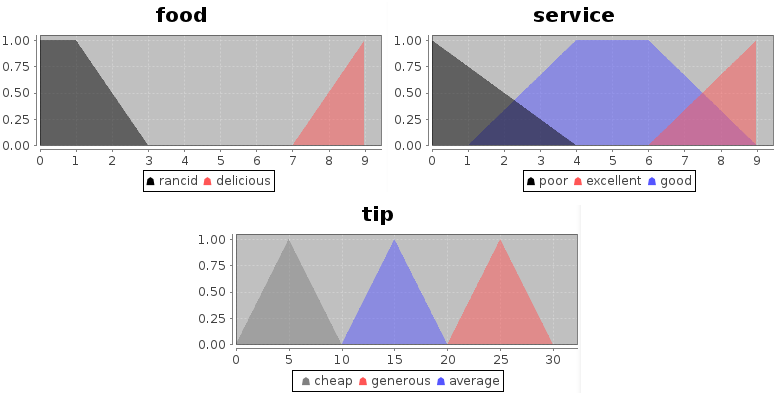
\includegraphics[width=3.1in]{./figs/tipper_MF.png}}
\vspace*{10pt}
\fcaption{Membership functions for tipper example.}\label{f:tipperMf}
\vspace*{10pt}

\begin{tiny}
\begin{alltt}
FUNCTION\_BLOCK tipper
VAR\_INPUT
\ 	service, food : REAL;
END\_VAR

VAR\_OUTPUT
\ 	tip : REAL;
END\_VAR

FUZZIFY service
\ 	TERM poor := (0, 1) (4, 0) ;
\ 	TERM good := (1, 0) (4,1) (6,1) (9,0);
\ 	TERM excellent := (6, 0) (9, 1);
END\_FUZZIFY

FUZZIFY food
\ 	TERM rancid := (0, 1) (1, 1) (3,0);
\ 	TERM delicious := (7,0) (9,1);
END\_FUZZIFY

DEFUZZIFY tip
\ 	METHOD : COG;			// Center of Gravity
\ 	TERM cheap := (0,0) (5,1) (10,0);
\ 	TERM average := (10,0) (15,1) (20,0);
\ 	TERM generous := (20,0) (25,1) (30,0);
END\_DEFUZZIFY

RULEBLOCK tipRules
\ 	Rule1: IF service IS poor OR food IS rancid 
\            THEN tip IS cheap;
\ 	Rule2: IF service IS good THEN tip IS average;
\ 	Rule3: IF service IS excellent AND food IS delicious 
\            THEN tip IS generous;
END\_RULEBLOCK
END\_FUNCTION\_BLOCK
\end{alltt}
\end{tiny}

A FIS inference system is usually composed of one or more Function Blocks (FB).
Every \texttt{FUNCTION\_BLOCK} has the following sections: i) input and output variables are define in \texttt{VAR\_INPUT} and \texttt{VAR\_OUTPUT} sections respectively; ii) fuzzification and defuzzification membership functions defined in \texttt{FUZZIFY} and \texttt{DEFUZZIFY} sections respectively; iii) fuzzy rules are written in the \texttt{RULEBLOCK} section.

Variable definition sections are straightforward, the variable name, type and possibly a default value are specified.

Membership functions either in \texttt{FUZZIFY} or \texttt{DEFUZZIFY} are defined for each linguistic term using the \texttt{TERM} statement followed by a function definition. 
In the previously shown example, functions are defined as piece-wise linear functions using series of points $(x_0,y_0) (x_1,y_1) ... (x_n, y_n)$. 
For instance \texttt{TERM average := (10,0) (15,1) (20,0)} defines a triangular membership function as shown (in blue) at the bottom of Figure~\ref{f:tipperMf}. 
Only two membership functions are defined in the IEC standard: singleton and piece-wise linear. 
As we shown in Section \ref{sec:jFu}, jFuzzyLogic significantly extends these concepts.

A FIS can contain one or more \texttt{RULEBLOCK}, where fuzzy rule sets are defined. 
Since rules are intrinsically parallel, no execution order is implied or warranted by the specified order in the program. 
Each rule is defined using standard ``\texttt{IF condition THEN conclusion  [WITH weight]}" clauses. 
The optional \texttt{WITH weight} statement allows weighting factors for each rule. 
Conditions tested in each \texttt{IF} clause are of the form ``\text{variable IS [NOT] linguistic\_term}". 
This test membership of \textit{variable} to a \textit{linguistic\_term} using the membership function defined in the corresponding \texttt{FUZZIFY} block.
An optional \text{NOT} operand negates the membership function (i.e. $\bar{m}(x) = 1 - m(x)$).
Obviously, several conditions can be combined using \texttt{AND} and \texttt{OR} connectors.

%--------------------------------------------------------------------------
\section{JFuzzyLogic \label{sec:jFu}}
%--------------------------------------------------------------------------

JFuzzyLogic's main goal is to facilitate and accelerate development of fuzzy systems.
We achieve this goal by:
i) using standard programming language (FCL) that reduces learning curves;
ii) providing a fully functional and complete implementation of fuzzy inference system (FIS);
iii) creating a programming interface (API) that developers can use or extend;
iv) implementing an Eclipse plugin to easily write and test FCL code;
v) making the software platform independent.
 and vi) distributing the software as open source. 
This allows to significantly accelerate development and testing of fuzzy systems in both industrial and academic environments.

In these sections we show how these design and implementation goals were achieved.
This should be particularly useful for developers and researchers looking to extend the functionality or use the available API.

\subsection{jFuzzyLogic Implementation \label{sec:implement}}

jFuzzyLogic is fully implemented in Java, thus the package is platform independent. 
ANTLR\cite{parr2007definitive} was used to generate Java code for a lexer and parser based on our FCL grammar definition.
This generated parser uses a left to right leftmost derivation recursive strategy, formally know as ``LL(*)".

Using the lexer and parser created by ANTLR we are able to parse FCL files by creating an Abstract Syntax Tree (AST), a well known structure in compiler design.
The AST is converted into an Interpreter Syntax Tree (IST), which is capable of performing the required computations.
This means that the IST can represent the grammar, like and AST, but it also capable of performing calculations.
The parsed FIS can be evaluated by recursively transversing the IST.

\subsection{Membership functions \label{sec:memFun}}

Only two membership functions are defined in the IEC standard: singleton and piece-wise linear.
jFuzzyLogic also implements other commonly used membership functions: 
\begin{itemize}
	\item Cosine : $ f(x | \alpha, \beta) = cos[\frac{\pi}{\alpha}(x - \beta)] , \forall x \in [-\alpha, \alpha]$
	\item Difference of sigmoidals: $f(x| \alpha_1, \beta_1, \alpha_2, \beta_2) = s(x,\alpha_1, \beta_1) - s(x,\alpha_2, \beta_2)$, where $s(x,\alpha, \beta) = 1 / [1+e^{-\beta (x-\alpha)}]$
	\item Gaussian : $f(x | \mu, \sigma) = e^{(x-\mu)^2 / 2 \sigma^2}$
	\item Gaussian double : $f(x | \mu_1, \sigma_1,\mu_2, \sigma_2) = $
\[
\left\lbrace \begin{array}{lr}
e^{(x-\mu_1)^2 / 2 \sigma_1^2} & x < \mu_1 \\
1 & \mu_1 \le x \le \mu_2 \\
e^{(x-\mu_2)^2 / 2 \sigma_2^2} & x > \mu_2 \\
\end{array}  \right.
\]
	\item Generalized bell : $f(x |\mu_1,a,b) = \frac{1}{1 + |(x-\mu)/a|^{2b}}$
	\item Sigmoidal : $f(x |\beta, t_0) = \frac{1}{1 + e^{\beta(x-t_0)}}$
	\item Trapezoidal : $f(x | m_{in}, l_{ow}, h_{igh}, m_{ax}) = $
\[
\left\lbrace \begin{array}{lr}
0 & x < m_{in} \\
\frac{x - m_{in} }{l_{ow} - m_{in} } & m_{in} \le x < l_{ow} \\
1 & l_{ow} \le x \le h_{igh} \\
\frac{x - h_{igh} }{m_{ax} - h_{igh} } & h_{igh} < x \le m_{ax} \\
0 & x > m_{ax} \\
\end{array}  \right.
\]
	\item Triangular: $f(x | m_{in}, m_{id}, m_{ax}) = $
\[
\left\lbrace \begin{array}{lr}
0 & x < m_{in} \\
\frac{x -m_{id} }{l_{ow} - m_{id} } & m_{in} \le x \le m_{id} \\
\frac{x - m_{id} }{m_{ax} - m_{id} } & m_{id} < x \le m_{ax} \\
0 & x > m_{ax} \\
\end{array}  \right.
\]
	\item Piece-wise linear : Defined as the union of all points by affine functions.
\end{itemize}

Furthermore, jFuzzyLogic allows to build arbitrary membership functions by combining mathematical expressions.
This is implemented by parsing an Interpreter Syntax Tree (IST) of mathematical expressions.
IST is evaluated at running time, thus allows including variables into the expressions.
Current implementation allows the use of the following functions:Abs, Cos, Exp, Ln, Log, Modulus, Nop, Pow, Sin, Tan, as well as addition, subtraction, multiplication and division.

\subsection{Aggregation, Activation \& Accumulation\label{sec:aggActAcc}}

As mentioned in section \ref{sec:FclConcepts}, rules are defined inside the \texttt{RULEBLOCK} statement in a FIS.
Each rule  block also specifies Aggregation, Activation and Accumulation methods.
All methods defined in the norm are implemented in jFuzzyLogic.
It should be noted that we adhere to the definitions of Aggregation, Activation and Accumulation as defined by IEC-61131-7, which may differ from the naming conventions from other references.

Aggregation methods (sometimes be called ``combination" or ``rule connection methods'') define the t-norms and t-conorms playing the role of AND \& OR operators, which can be:

\begin{scriptsize}
\begin{center}
\begin{tabular}{|l|l|l|}
\hline 
Name & x AND y & x OR y \\ 
\hline 
Min/Max & $min(x,y)$ & $max(x,y)$ \\ 
\hline 
Bdiff/Bsum & $max(0,x+y-1)$ & $min(1,x+y)$ \\ 
\hline 
Prod/PobOr & $x \; y$ & $x + y - x \; y$ \\ 
\hline 
Drastic & if$(x==1) \rightarrow y$  & if$(x==0) \rightarrow y$ \\ 
        & if$(y==1) \rightarrow x$  & if$(y==0) \rightarrow x$ \\ 
        & otherwise $\rightarrow 0$ & otherwise $\rightarrow 1$ \\ 
\hline 
Nil potent & if$( x+y > 1) \rightarrow min(x,y)$  & if$( x+y < 1) \rightarrow max(x,y)$   \\ 
           & otherwise $\rightarrow 0$            & otherwise $\rightarrow 1$ \\ 
\hline 
\end{tabular} 
\end{center}
\end{scriptsize}

Needless to say, each set of operators must satisfy De Morgan’s laws.

Activation method define how rule antecedents modify rule consequents, i.e. once the IF part has been evaluated, how this result is applied to the THEN part of the rule.  
The most common activation operators are Minimum and Product (see Figure~\ref{f:activation}).
Both methods are implemented in jFuzzyLogic.

\vspace*{10pt}
\centerline{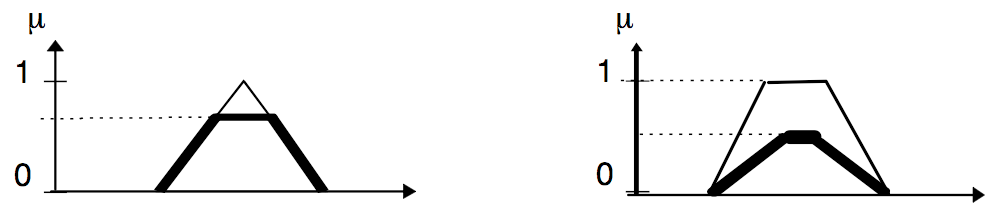
\includegraphics[width=3.1in]{./figs/MaxProd.png}}
\vspace*{10pt}
\fcaption{Activation methods: Min (left) and Prod (right).}\label{f:activation}
\vspace*{10pt}

Finally, accumulation method defines how the consequents from multiple rules are combined within a Rule Block (see Figure~\ref{f:acumulation}).
Accumulation methods implemented by jFuzzyLogic defined in the norm include: 

\begin{itemize}
	\item Maximum : $\alpha_{cc} = max(\alpha_{cc}, \delta)$
	\item Bounded sum: $\alpha_{cc} = min(1, \alpha_{cc} + \delta)$
	\item Normalized sum: $\alpha_{cc} = \frac{\alpha_{cc} + \delta}{max(1, \alpha_{cc} + \delta)}$
	\item Probabilistic OR : $\alpha_{cc} =  \alpha_{cc} + \delta -  \alpha_{cc} \; \delta$
\end{itemize}

where $\alpha_{cc}$ is the accumulated value (at point $x$) and $\delta = m(x)$ is the membership function for defuzzification (also at $x$).

\vspace*{10pt}
\centerline{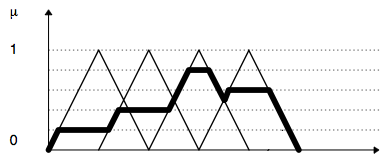
\includegraphics[width=3.1in]{./figs/accumulation.png}}
\vspace*{10pt}
\fcaption{Accumulation method: Combining consequents from multiple rules using ‘Max’ accumulation method.}\label{f:acumulation}
\vspace*{10pt}

\subsection{Defuzzification\label{sec:defuzz}}

In case of simple membership functions, such as trapezoidal and piece-wise linear, defuzzicication can be computed easily by applying know mathematical equations.
Although it can be done very efficiently, unfortunately it cannot be generalized to arbitrary expressions.

Due to the flexibility in defining membership functions, we use a more general method.
We discretize membership functions at a number of points and use a , more computational intensive, numerical integration method.
The number of points used for discretization, by default one thousand, can be adjusted according to the precision-speed trade-off required for a particular application.
Inference is performed by evaluating membership functions at these discretization points.
In order to perform a discretization, the ``universe" for each variable, has to be estimated. 
The universe is defined as the range where the variable has non-neglectable value. 
For each variable, each membership function and each term is taken into account when calculating a universe.
Once all rules have been analyzed, the accumulation for each variable is complete. 

The last step when evaluating a FIS is defuzzification.
The value for each variable is calculated using the selected defuzzification method, which can be:

\begin{itemize}
	\item Center of gravity : $\frac{\int{x \mu(x) dx}}{\int{\mu(x) dx}}$
	\item Center of gravity singleton : $\frac{\sum_{i}{x_i \mu_i}}{\sum_{i}{\mu_i}}$
	\item Center of area : $u \; | \; \int_{-\infty}^{u}{\mu(x) dx} = \int_{u}^{\infty}{\mu(x) dx}$
	\item Rightmost Max : $arg\max_{x}{[ \mu(x) = max(\mu(x)) ] }$
	\item Leftmost Max : $arg\min_{x}{[ \mu(x) = max(\mu(x)) ] }$
	\item Mean max : $mean(x) \; | \; \mu(x) = max(\mu(x)) $
\end{itemize}


\subsection{API extensions \label{sec:ext}}

Some of the extensions and benefits provided by jFuzzyLogic are described in this section.

\textit{Modularity.} Modular design allows to extend the language and the API easily. It is possible to add custom aggregation, activation or accumulation methods, defuzzifiers, or membership functions by extending the provided object tree (see Figure~\ref{f:acumulation}). 


\textit{Dynamic changes.} Our API supports dynamic changes made onto a fuzzy inference system: i) variables can be used as membership function parameters; ii) rules can be added or deleted from rule blocks, iii) rule weights can be modified; iv) membership functions can use combinations of pre-defined functions. 

\textit{Data Types.} Due to the nature of fuzzy systems and in order to reduce complexity, jFuzzyLogic considers each variable as \textit{REAL} variable which is mapped to a \textit{double} Java type.

\textit{Excecution order.} By default it is assumed that a FIS is composed of only one Function Block, so evaluating the FIS means evaluating the default FB. 
If a FIS has more than one FB, they are evaluated in alphabetical order by FB name. 
Other execution orders can be implemented by the user, which allows us to easily define hierarchical controllers.

\vspace*{10pt}
\centerline{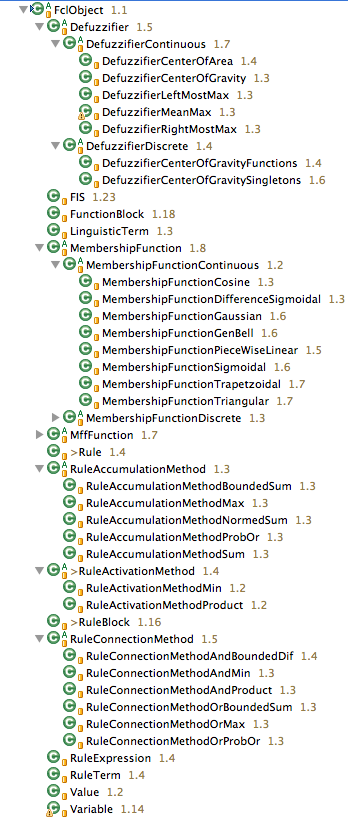
\includegraphics[width=2.9in]{./figs/jFuzzy_object_tree.png}}
\vspace*{10pt}
\fcaption{jFuzzyLogic object tree provides many extension points.}\label{f:acumulation}
\vspace*{10pt}

%--------------------------------------------------------------------------
\subsection{Optimization API \label{sec:optim}}
%--------------------------------------------------------------------------

An optimization API was developed in order to automatically fine tune FIS parameters.
Our goal was to define a very lightweight and easy to learn API, which was flexible enough to be extended for general purpose usage.

The most common parameters to be optimized are membership functions and rule weights.
For instance if a variable has a fuzzifier term ``\texttt{TERM rancid := TRIAN 0 1 3}", there are three parameters that can be optimized in this membership function (whose initial values are 0, 1 and 3 respectively). 
Using the API, we can choose to optimize any of subset of them.
Similarly, in the rule ``\texttt{IF service IS good THEN tip IS average}" we can optimize the weight of this rule (implicit ``\text{WITH 1.0}" statement).

The API, is composed of the following objects:

\begin{itemize}
	\item \textit{ErrorFunction} : An object that evaluates a Rule Block and calculates the error. 
		Extending ErrorFunction is the bare minimum required to implement an optimization using one of the available optimization methods.

	\item \textit{OptimizationMethod} : An optimization method object is an abstraction of an algorithm. It changes \textit{Parameter} based on the performance measured using an ErrorFunction.

	\item \textit{Parameter} : This class represents a parameter to be optimized. 
		Any change on a parameter, will perform the corresponding change on the FIS, thus changing the outcome.
		There are two basic parameters: ParameterMembershipFunction and ParameterRuleWeight which allows for changes in membership functions and rule weights respectively. 
		Other parameters could be created, for instance, in order to completely rewrite rules. 
		We plan to extend them in future releases. 
		Most users will not need to extend \textit{Parameter} objects.

\end{itemize}

For most optimization applications, extending only one or two objects is enough (i.e. \textit{ErrorFunction}, and sometimes \textit{OptimizationMethod}).
We provide template and demo objects to show how this can be done, all of them are included in our freely available source code.

A few optimization algorithms are implemented, such as gradient descent, partial derivative, and delta algorithm.
As we mentioned, other algorithms can be easily implemented based on these templates or by directly extending them.
In the provided examples it is assumed that error functions can be evaluated anywhere in the input space.
Obviously, such evaluation is usually not available in real world applications, otherwise we would probably not need to implement a fuzzy system.
This is not a limitation in the API, since we can always develop an optimization algorithm and the corresponding error function that evaluates the FIS on a learning set.


%--------------------------------------------------------------------------
\section{Eclipse plugin\label{sec:pluggin}}
%--------------------------------------------------------------------------

Eclipse is one of the most commonly used software development platforms.
It allows to specific language development tool by using the Eclipse-plugin framework.
We developed a jFuzzyLogic plugin that allows developers to easily and rapidly write FCL code, and test it.
Our plugin was developed using Xtext, a well known framework for domain specific languages based on ANTLR.

The plugin supports several features, such as syntax coloring, content assist, validation, program outlines and hyperlinks for variables and linguistic terms, etc.
Figure \ref{f:pluginEdit} shows an example of the plugin being used to edit FCL code, the left panel shows an editor providing syntax coloring while adding content assist at cursor position, the right panel shows the corresponding code outline. 

Running an FCL program (Figure \ref{f:pluginRun}) shows membership functions for all input and output variables while output console shows the FCL code parsed by jFuzzyLogic.

\vspace*{10pt}
\centerline{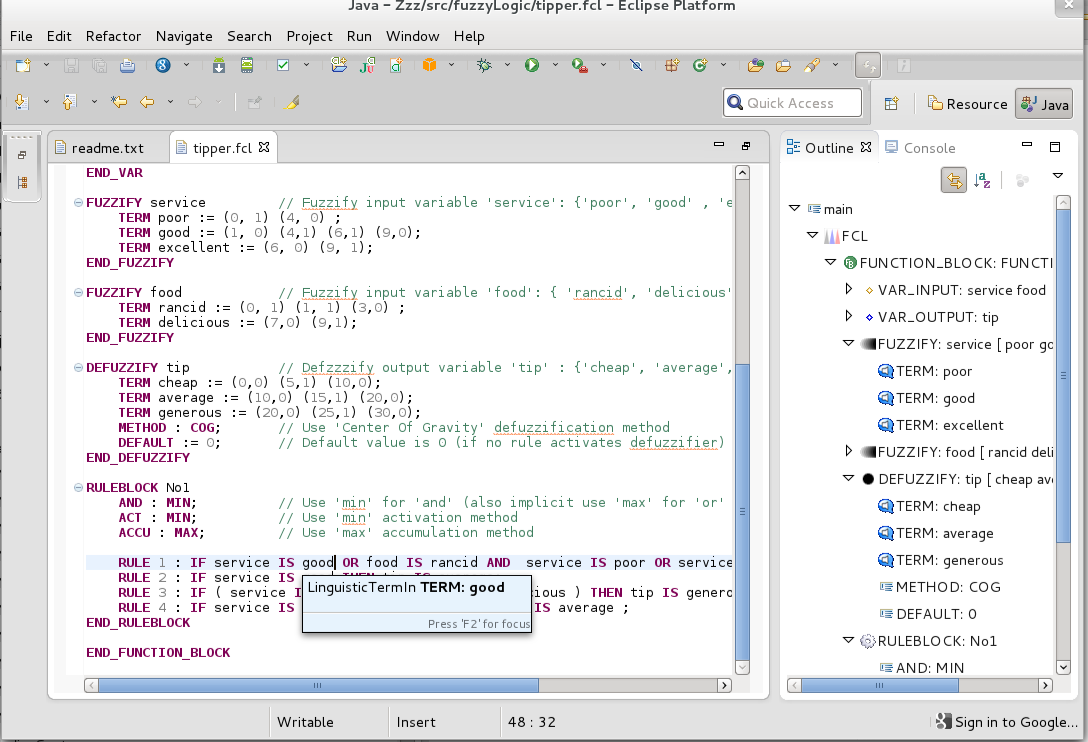
\includegraphics[width=2.9in]{./figs/plugin_edit}}
\vspace*{10pt}
\fcaption{jFuzzyLogic plugin for Eclipse. The editor (left window) provides syntax coloring and content assist. The right window shows code outline.}\label{f:pluginEdit}
\vspace*{10pt}

\vspace*{10pt}
\centerline{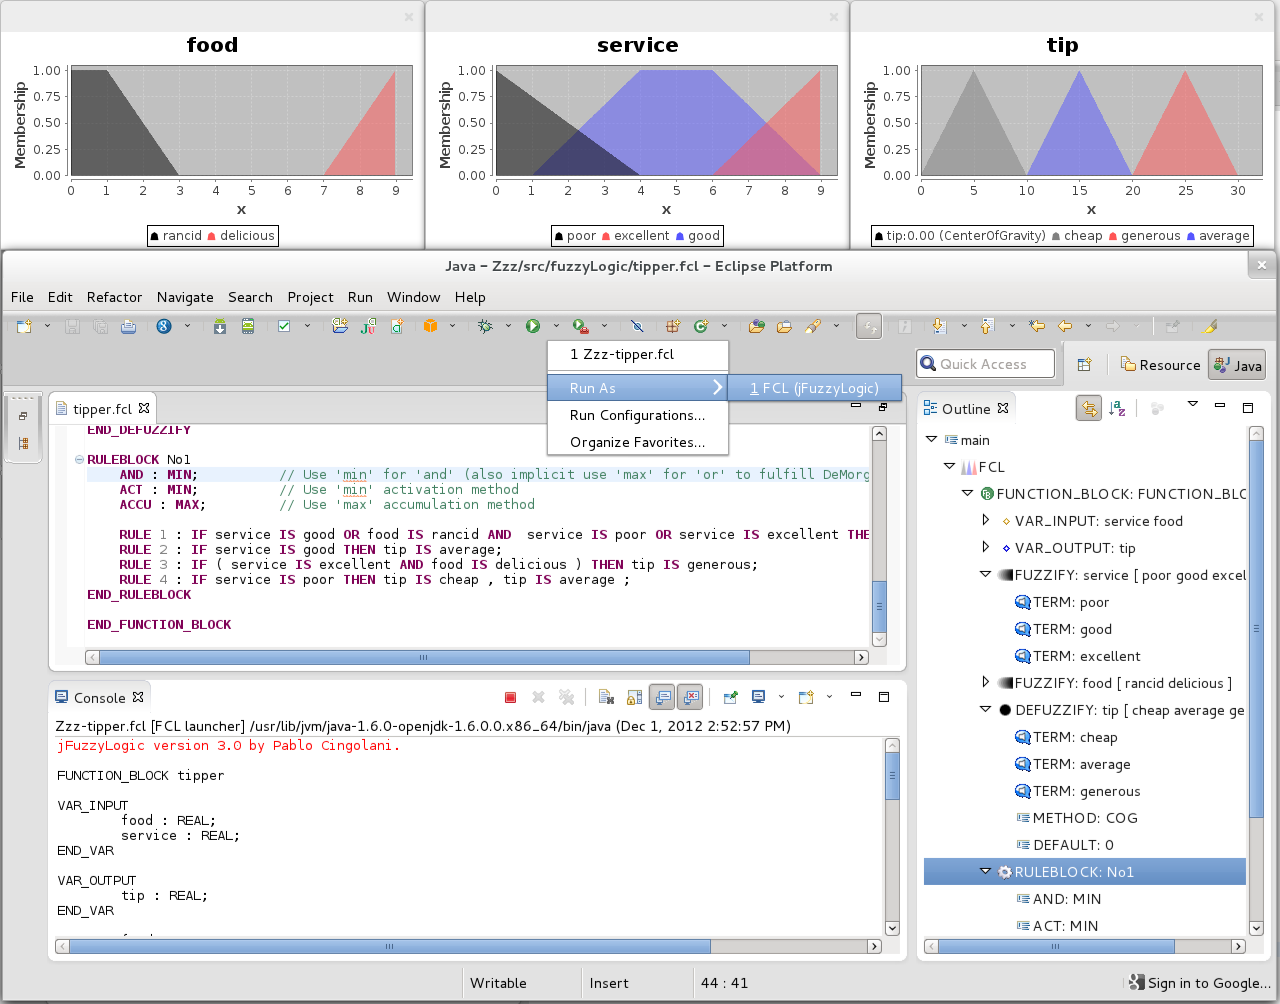
\includegraphics[width=2.9in]{./figs/plugin_run}}
\vspace*{10pt}
\fcaption{jFuzzyLogic plugin for Eclipse. Running an FCL program (Figure \ref{f:pluginRun}) shows membership functions for all input and output variables.}\label{f:pluginRun}
\vspace*{10pt}


%--------------------------------------------------------------------------
\section{A case study\label{sec:cas}}
%--------------------------------------------------------------------------

We present an example of creating an FLC controller with jFuzzyLogic. 
This case study is focused on the development of the wall following robot as explained in \cite{mucientes2009learning}. 
Wall following behavior is well known in mobile robotics. 
It is frequently used for the exploration of unknown indoor environments and for the navigation between two points in a map. 


The main requirement of a good wall-following controller is to maintain a suitable distance from the wall that is being followed. 
The robot should also move as fast as possible, while avoiding sharp movements, making smooth and progressive turns and changes in velocity.

In our fuzzy control system, the input variables are: 
	i) normalized distances from the robot to the right ($RD$) and left walls ($DQ$); 
	ii) orientation with respect to the wall ($O$); and 
	iii) linear velocity ($V$). 

The output variables in this controller are the normalized linear acceleration ($LA$) and the angular velocity ($AV$). 
The linguistic partitions are shown in Figure~\ref{f:robotVars} which are comprised by linguistic terms with uniformly distributed triangular membership functions giving meaning to them.

\vspace*{10pt}
\centerline{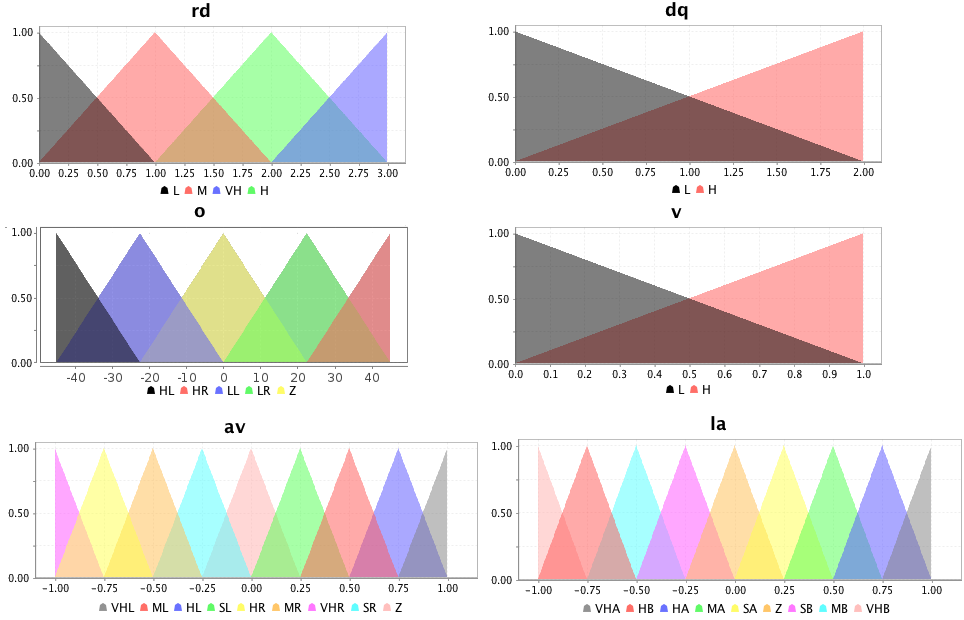
\includegraphics[width=3.1in]{./figs/robot_vars_2.png}}
\vspace*{10pt}
\fcaption{Membership functions for wall-following robot.}\label{f:robotVars}
\vspace*{10pt}

In order to implement the controller, the first step is to declare the input and output variables and to define the fuzzy sets. 
Variables are defined in \textit{VAR\_INPUT} and \textit{VAR\_OUTPUT} sections. 
Fuzzy sets are defined in \textit{FUZZIFY} blocks for input variables and \textit{DEFUZZIFY} blocks for output variables.

One \textit{FUZZIFY} block is used for each input variable. 
Each \textit{TERM} line within a \textit{FUZZIFY} block defines a linguistic term and its corresponding membership function.
In this example all membership functions are triangular, so they are defined using the \textit{'trian'} keyword, followed by three parameters defining left, center and right points (e.g. \textit{`TRIAN 1 2 3'}).

Output variables define their membership functions within \textit{DEFUZZIFY} blocks. 
Linguistic terms and membership functions are defined using the \textit{TERM} keyword as previously described for input variables. 
In this case we also add parameters to select the defuzzyfication method. 
The statement \textit{'METHOD : COG'} indicates that we are using 'Center of gravity'. 
The corresponding FCL code generated for the first step is as follows:

\vspace*{10pt}
\begin{scriptsize}
\begin{alltt}
VAR\_INPUT
\ 	rd : REAL;			// Right distance
\ 	dq : REAL;			// Distance quotient
\ 	o  : REAL;			// Orientation
\ 	v  : REAL;			// Velocity
END\_VAR

VAR\_OUTPUT
\ 	la : REAL;			// Linear acceleration
\ 	av : REAL;			// Angular velocity
END\_VAR

FUZZIFY rd
\ 	TERM L  := TRIAN 0 0 1;
\ 	TERM M  := TRIAN 0 1 2;
\ 	TERM H  := TRIAN 1 2 3;
\ 	TERM VH := TRIAN 2 3 3;
END\_FUZZIFY

FUZZIFY dq
\ 	TERM L := TRIAN 0 0 2;
\ 	TERM H := TRIAN 0 2 2;
END\_FUZZIFY

FUZZIFY o
\ 	TERM HL := TRIAN -45 -45 -22.5;
\ 	TERM LL := TRIAN -45 -22.5 0;
\ 	TERM Z  := TRIAN -22.5 0 22.5;
\ 	TERM LR := TRIAN 0 22.5 45;
\ 	TERM HR := TRIAN 22.5 45 45;
END\_FUZZIFY

FUZZIFY v
\ 	TERM L := TRIAN 0 0 1;
\ 	TERM H := TRIAN 0 1 1;
END\_FUZZIFY

DEFUZZIFY la
\ 	TERM VHB := TRIAN -1 -1 -0.75;
\ 	TERM HB  := TRIAN -1 -0.75 -0.5;
\ 	TERM MB  := TRIAN -0.75 -0.5 -0.25;
\ 	TERM SB  := TRIAN -0.5 -0.25 0;
\ 	TERM Z   := TRIAN -0.25 0 0.25;
\ 	TERM SA  := TRIAN 0 0.25 0.5;
\ 	TERM MA  := TRIAN 0.25 0.5 0.75;
\ 	TERM HA  := TRIAN 0.5 0.75 1;
\ 	TERM VHA := TRIAN 0.75 1 1;
\ 	METHOD : COG;			// Center of Gravity
\ 	DEFAULT := 0;
END\_DEFUZZIFY

DEFUZZIFY av
\ 	TERM VHR := TRIAN -1 -1 -0.75;
\ 	TERM HR  := TRIAN -1 -0.75 -0.5;
\ 	TERM MR  := TRIAN -0.75 -0.5 -0.25;
\ 	TERM SR  := TRIAN -0.5 -0.25 0;
\ 	TERM Z   := TRIAN -0.25 0 0.25;
\ 	TERM SL  := TRIAN 0 0.25 0.5;
\ 	TERM ML  := TRIAN 0.25 0.5 0.75;
\ 	TERM HL  := TRIAN 0.5 0.75 1;
\ 	TERM VHL := TRIAN 0.75 1 1;
\ 	METHOD : COG;
\ 	DEFAULT := 0;
END\_DEFUZZIFY
\end{alltt}
\end{scriptsize}

\vspace*{10pt}
These membership functions can be plotted by running jFuzzyLogic with the FCL file generated as argument (e.g. \texttt{java -jar jFuzzyLogic.jar robot.fcl}). 
The corresponding FCL file for this case study is available for download as one of the examples provided in jFuzzyLogic package (\texttt{jfuzzylogic.sourceforge.net}).

The second step is to define the rules used for inference. 
They are defined in \textit{RULEBLOCK} statements. 
For the wall-following robot controller, we used 'minimum' connection method (\textit{AND : MIN}), minimum activation method (\textit{ACT : MIN}), and maximum accumulation method (\textit{ACCU : MAX}). 
We implemented the rule base generated in~\cite{mucientes2009learning} by the WCOR method~\cite{Alc06}. 
Each entry in the rule base was converted to a single FCL rule. 
Within each rule, the antecedent (i.e. the \textit{IF} part) is composed of the input variables connected by \textit{`AND'} operators. 
Since there are more than one output variable, we can specify multiple consequents (i.e. \textit{THEN} part) separated by semicolons. 
Finally, we add the desired weight using the \textit{`with'} keyword followed by the weight. 
This completes the implementation of a controller for a wall-following robot using FCL and jFuzzyLogic. 
The Java code generated for the second step is as follows:

\vspace*{10pt}
\begin{scriptsize}
\begin{alltt}
RULEBLOCK rules
AND  : MIN;			// Use 'min' for 'and' (also implicit use 
            //'max' for 'or' to fulfill DeMorgan's Law)
ACT  : MIN;			// Use 'min' activation method
ACCU : MAX;			// Use 'max' accumulation method

RULE 01: IF rd is  L and dq is L and o is LL 
    and v is L THEN la is VHB , av is VHR with 0.4610;
RULE 02: IF rd is  L and dq is L and o is LL 
    and v is H THEN la is VHB , av is VHR with 0.4896;
RULE 03: IF rd is  L and dq is L and o is  Z 
    and v is L THEN la is   Z , av is  MR with 0.6664;
RULE 04: IF rd is  L and dq is L and o is  Z 
    and v is H THEN la is  HB , av is  SR with 0.5435;
RULE 05: IF rd is  L and dq is H and o is LL 
    and v is L THEN la is  MA , av is  HR with 0.7276;
RULE 06: IF rd is  L and dq is H and o is  Z 
    and v is L THEN la is  MA , av is  HL with 0.4845;
RULE 07: IF rd is  L and dq is H and o is  Z 
    and v is H THEN la is  HB , av is  ML with 0.5023;
RULE 08: IF rd is  L and dq is H and o is LR 
    and v is H THEN la is VHB , av is VHL with 0.7363;
RULE 09: IF rd is  L and dq is H and o is HR 
    and v is L THEN la is VHB , av is VHL with 0.9441;
RULE 10: IF rd is  M and dq is L and o is  Z 
    and v is H THEN la is  SA , av is  HR with 0.3402;
RULE 11: IF rd is  M and dq is L and o is LR 
    and v is H THEN la is   Z , av is VHL with 0.4244;
RULE 12: IF rd is  M and dq is L and o is HR 
    and v is L THEN la is  SA , av is  HL with 0.5472;
RULE 13: IF rd is  M and dq is L and o is HR 
    and v is H THEN la is  MB , av is VHL with 0.4369;
RULE 14: IF rd is  M and dq is H and o is HL 
    and v is L THEN la is   Z , av is VHR with 0.1770;
RULE 15: IF rd is  M and dq is H and o is HL 
    and v is H THEN la is VHB , av is VHR with 0.4526;
RULE 16: IF rd is  M and dq is H and o is LL 
    and v is H THEN la is  SA , av is VHR with 0.2548;
RULE 17: IF rd is  M and dq is H and o is  Z 
    and v is L THEN la is  HA , av is   Z with 0.2084;
RULE 18: IF rd is  M and dq is H and o is LR 
    and v is L THEN la is  HA , av is VHL with 0.6242;
RULE 19: IF rd is  M and dq is H and o is LR 
    and v is H THEN la is  SA , av is VHL with 0.3779;
RULE 20: IF rd is  M and dq is H and o is HR 
    and v is L THEN la is   Z , av is VHL with 0.6931;
RULE 21: IF rd is  M and dq is H and o is HR 
    and v is H THEN la is VHB , av is VHL with 0.7580;
RULE 22: IF rd is  H and dq is L and o is  Z 
    and v is L THEN la is  HA , av is VHR with 0.5758;
RULE 23: IF rd is  H and dq is L and o is LR 
    and v is H THEN la is  SA , av is  MR with 0.2513;
RULE 24: IF rd is  H and dq is L and o is HR 
    and v is L THEN la is  HA , av is VHL with 0.5471;
RULE 25: IF rd is  H and dq is L and o is HR 
    and v is H THEN la is  SA , av is  HL with 0.5595;
RULE 26: IF rd is  H and dq is H and o is HL 
    and v is L THEN la is VHB , av is VHR with 0.9999;
RULE 27: IF rd is  H and dq is H and o is HL 
    and v is H THEN la is VHB , av is VHR with 0.9563;
RULE 28: IF rd is  H and dq is H and o is LL 
    and v is L THEN la is  HA , av is VHR with 0.9506;
RULE 29: IF rd is  H and dq is H and o is  Z 
    and v is L THEN la is  HA , av is VHR with 0.4529;
RULE 30: IF rd is  H and dq is H and o is  Z 
    and v is H THEN la is  SA , av is VHR with 0.2210;
RULE 31: IF rd is  H and dq is H and o is LR 
    and v is L THEN la is  HA , av is  MR with 0.3612;
RULE 32: IF rd is  H and dq is H and o is LR 
    and v is H THEN la is  SA , av is  MR with 0.2122;
RULE 33: IF rd is  H and dq is H and o is HR 
    and v is L THEN la is  HA , av is  HL with 0.7878;
RULE 34: IF rd is  H and dq is H and o is HR 
    and v is H THEN la is  SA , av is VHL with 0.3859;
RULE 35: IF rd is VH and dq is L and o is LR 
    and v is L THEN la is  HA , av is VHR with 0.5530;
RULE 36: IF rd is VH and dq is L and o is HR 
    and v is L THEN la is  HA , av is  HR with 0.4223;
RULE 37: IF rd is VH and dq is L and o is HR 
    and v is H THEN la is  SA , av is  HR with 0.3854;
RULE 38: IF rd is VH and dq is H and o is LL 
    and v is L THEN la is  HA , av is VHR with 0.0936;
RULE 39: IF rd is VH and dq is H and o is LR 
    and v is L THEN la is  HA , av is VHR with 0.7325;
RULE 40: IF rd is VH and dq is H and o is LR 
    and v is H THEN la is  SA , av is VHR with 0.5631;
RULE 41: IF rd is VH and dq is H and o is HR 
    and v is L THEN la is  HA , av is  HR with 0.5146;
END\_RULEBLOCK
\end{alltt}
\end{scriptsize}
\vspace*{10pt}

\vspace*{10pt}
The corresponding Java code that use jFuzzyLogic for running the FCL generated will be:
\\
\begin{scriptsize}
\begin{alltt}
public class TestRobot \{
  public static void main(String[] args) 
  throws Exception \{
    FIS fis = FIS.load("fcl/robot.fcl", true);
    FunctionBlock fb = fis.getFunctionBlock(null);
    // Set inputs
    fb.setVariable("rd", 0.3); 
    fb.setVariable("dq", 1.25);
    fb.setVariable("o", 2.5); 
    fb.setVariable("v", 0.6);
    // Evaluate
    fb.evaluate(); 
    // Get output
    double la = fb.getVariable("la").getValue());
    double av = fb.getVariable("av").getValue());
  \}
\}
\end{alltt}
\end{scriptsize}


This can also be done using the command line option ``-e", which assigns values in the command line to input variables alphabetically (in this case: ``dp", ``o", ``rd" and ``v") and then evaluates the FIS. 
This utility produces plots of memnbership functions for all variables, as well as deffuzification areas for output all variables, in this example, ``av" and ``la" shown in light grey in Figure \ref{f:robot_out}).
Here we show the command, as well as part of the output:
\\
\begin{scriptsize}
\begin{alltt}
\$ java -jar jFuzzyLogic.jar -e robot.fcl \textbackslash
      1.25 2.5 0.3 0.6

FUNCITON_BLOCK robot
\ 	VAR_INPUT 	        dq = 1.250000
\ 	VAR_INPUT 	         o = 2.500000
\ 	VAR_INPUT 	        rd = 0.300000
\ 	VAR_INPUT 	         v = 0.600000
\ 	VAR_OUTPUT	        av = 0.061952
\ 	VAR_OUTPUT	        la = -0.108399
\   ...(rule activations omitted)
\end{alltt}
\end{scriptsize}

\vspace*{10pt}
\centerline{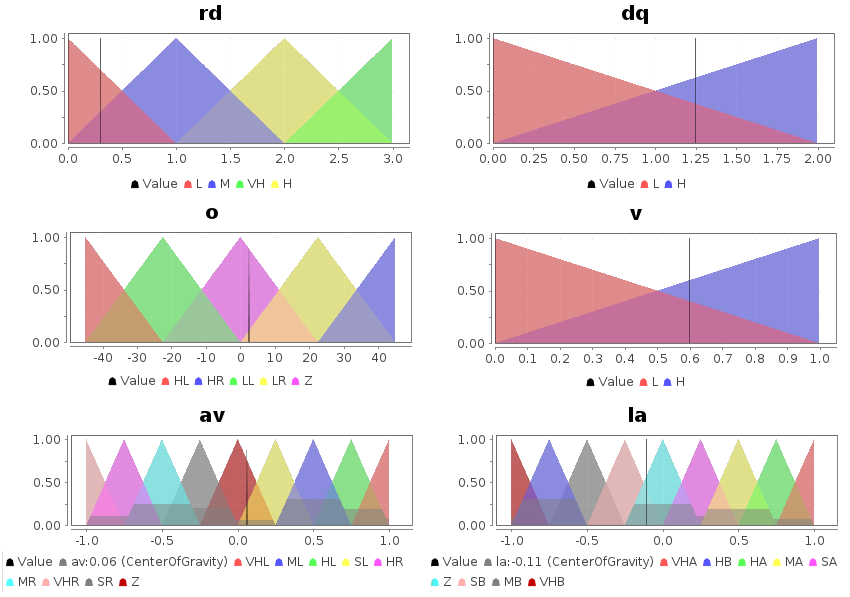
\includegraphics[width=2.9in]{./figs/robot_out2.png}}
\vspace*{10pt}
\fcaption{Memnbership functions and deffuzification areas (light grey) for \texttt{robots.fcl} example.}\label{f:robot_out}
\vspace*{10pt}


%--------------------------------------------------------------------------
\section{Conclusions \label{sec:con}}
%--------------------------------------------------------------------------

In this paper, we have described jFuzzyLogic, an open source Java library for fuzzy systems which allow us to design FLCs following the standard IEC 61131.
It allows us to reduce programming work and extend the range of possible users applying fuzzy systems and FLCs.

We have shown a case study to illustrate the use of jFuzzyLogic. 
In this case, we developed an FLC controller for wall-following behavior in a robot.
The example shows how FCL can be used to easily implement fuzzy logic systems.

The jFuzzyLogic software package is continuously being updated and improved. 
At the moment, we are developing an implementation of a C++ compiler for fuzzy inference systems. 
This will allow easy implementation with embedded control systems using different processors.

%--------------------------------------------------------------------------
\section*{Acknowledgments}
%--------------------------------------------------------------------------

jFuzzyLogic was designed and developed by P. Cingolani. He is supported in part by McGill Uninversity, Genome Quebec. 
J. Alcala-Fdez is supported by the Spanish Ministry of Education and Science under Grant TIN2011-28488 and the Andalusian Government under Grant P10-TIC-6858.
We would like to thank M. Blanchette and R. Sladek for their comments.


%--------------------------------------------------------------------------
\section*{References}
%--------------------------------------------------------------------------

\bibliographystyle{unsrt}
\bibliography{CingolaniAlcala-Fdez-IJCIS2012}

\end{multicols}
\end{document}
